% Needed packages
\documentclass[a4paper, 10pt, english, onecolumn]{article}
\usepackage[english]{babel}
\usepackage[cm]{fullpage}
\usepackage{cite}
\usepackage{anysize}
\usepackage{setspace}
%\usepackage[compact]{titlesec}
\usepackage{graphicx}
\usepackage{stfloats}
\usepackage{listings}
\usepackage{hyperref}

\usepackage{amssymb,amsmath}
\usepackage{algorithmicx}
%\usepackage{algorithmic}
\usepackage{algorithm}
\usepackage[noend]{algpseudocode}

% for coloring individual cells in a table
\usepackage[table]{xcolor}
%\usepackage{pgfgantt}

%\newcommand{\keywords}[1]{\par\noindent 
%{\bf Keywords\/}. #1}

% Margins & Headers
\marginsize{2.5cm}{2.5cm}{3.0cm}{2.0cm}
\columnsep 0.4in
\footskip 0.4in 
\usepackage{changepage}

% E-mail formatting
\usepackage{color,hyperref}
    \catcode`\_=11\relax
    \newcommand\email[1]{\_email #1\q_nil}
    \def\_email#1@#2\q_nil{
      \href{mailto:#1@#2}{{\emailfont #1\emailampersat #2}}
    }
    \newcommand\emailfont{\sffamily}
    \newcommand\emailampersat{{\color{red}\small@}}
    \catcode`\_=8\relax 
	
% List modifications
\newenvironment{packed_item}{
\begin{itemize}
  \setlength{\itemsep}{1pt}
  \setlength{\parskip}{0pt}
  \setlength{\parsep}{0pt}
}{\end{itemize}}

\newenvironment{packed_enum}{
\begin{enumerate}
  \setlength{\itemsep}{1pt}
  \setlength{\parskip}{0pt}
  \setlength{\parsep}{0pt}
}{\end{enumerate}}

% ### Mathematics ###
\newcommand{\bpm}{\begin{pmatrix}}
\newcommand{\epm}{\end{pmatrix}}

\newcommand{\bbm}{\begin{bmatrix}}
\newcommand{\ebm}{\end{bmatrix}}

\newcommand{\bsm}{\bigl( \begin{smallmatrix}}
\newcommand{\esm}{ \end{smallmatrix} \bigl)} 

\newcommand{\mbf}{\mathbf}

% ### Matrices and Vectors ###
\newcommand{\mtx}[1]{\ensuremath{\boldsymbol{#1}}}
\newcommand*\Let[2]{\State #1 $\gets$ #2}

% ### Sets ###
\newcommand{\set}[1]{\ensuremath{\mathcal{#1}}}

% ### Other ###

\newcommand{\transpose}{^{T}}
\newcommand{\inv}{^{-1}}
\newcommand{\pseudoinv}{^{+}}

% ### Hyphenation ###
\hyphenation{a-na-ly-sis}

% ### dots at the end of arrows and lines ###

\def \orightarrow {\circ\hspace{-0.42em}\rightarrow}
\def \oleftarrow {\leftarrow\hspace{-0.42em}\circ}
\def \orightline {\circ\hspace{-0.16em}-}
\def \oleftline {-\hspace{-0.16em}\circ}
\def \oline {\circ\hspace{-0.38em}-\hspace{-0.2em}\circ}
\def \srightarrow {\text{\textasteriskcentered}\hspace{-0.62em}\rightarrow}
\def \sleftarrow {\leftarrow\hspace{-0.62em}\text{\textasteriskcentered}}
\def \srightline {\text{\textasteriskcentered}\hspace{-0.16em}-}
\def \sleftline {-\hspace{-0.40em}\text{\textasteriskcentered}}
\def \sline {\text{\textasteriskcentered}\hspace{-0.38em}-\hspace{-0.4em}\text{\textasteriskcentered}}
\def \soline {\text{\textasteriskcentered}\hspace{-0.16em}-\hspace{-0.4em}\circ}
\def \osline {\circ\hspace{-0.38em}-\hspace{-0.16em}\text{\textasteriskcentered}}

% ############## End Macros ##############

% ### Section Formatting ###
\usepackage[compact]{titlesec}
\titlespacing*{\section}{4pt}{*0}{4pt}

% ### Paragraph Formatting ###
\makeatletter
\renewcommand{\paragraph}{%
  \@startsection{paragraph}{4}%
  {\z@}{0.5ex \@plus 1ex \@minus .2ex}{-1em}%
  {\normalfont\normalsize\bfseries}%
}
\makeatother

% Title
\title{\fontfamily{phv}\selectfont{Causal Discovery methods for Effective Connectivity in Human Brains}}
\author{
  \textbf{R. Janssen} - \href{mailto:ramon.janssen@student.ru.nl}{ramon.janssen@student.ru.nl} \\
  \textbf{T. de Ruijter} - \href{mailto:t.deruijter@student.ru.nl}{t.deruijter@student.ru.nl}\\
%  \textbf{T. Claassen} - \href{mailto:tomc@cs.ru.nl}{tomc@cs.ru.nl}\\
%  \textbf{M. Hinne} - \href{mailto:mhinne@cs.ru.nl}{mhinne@cs.ru.nl}
}

\date{\fontfamily{ptm}\selectfont{\small{\bfseries{\today - Radboud
Universiteit Nijmegen}}}\\[0.5cm]\rule{\linewidth}{0.3mm}}

\begin{document}

\maketitle

\setlength{\parindent}{0.0cm}
\setlength{\parskip}{3mm plus2mm minus1.5mm}

\begin{abstract}
Many different approaches have been used to infer brain connectivity.
But few general causal discovery methods have yet been used to find effective connectivity.
In this article, we describe how the PC algorithm is used on functional brain-data.
This approach results in connectivity matrices which clearly show some well-known brain connections.
Some disadvantages of the PC algorithm for this use are discussed, and an attempt is made to decrease these disadvantages by making adjustments to the algorithm.
Causal relations have only be found with very low certainty. 
%In this work we applied PC algorithm on resting-state data of healthy human subjects.
%Additionally we propose a variant of PC algorithm that poses weaker assumptions on the model, better fitting the underlying model.
%We find that detecting structure homological areas in the brain works better with PC algorithm than most conventional diffusion weighted imaging techniques.
%In the area of directionality and causality, more research is needed.
\end{abstract}

\section{Introduction}
% Subject introduction
The brain and particularly the human brain have been studied for hundreds of years.
Today, brain research is still one of the thriving fields of research.
A lot has changed since the time of Phrenology, the pseudoscience attempting to derive cognitive ability and personality from measurements of the skull or, post-mortem, the brain.
Advanced and non-intrusive measurement methods exist that allow scientists to peek inside brains that give a coarse but broad overview, with widespread established clinical and research purposes.

% Motivation for brain connectomics
The question how our brains are wired - brain connectomics - drives one of the main fields of research in neuroscience.
Our brains are in essence networks which can be analysed similarly to very large graphs.
That is why it is almost natural to apply graphical modelling methods to brain data.
The field of brain connectivity finds its roots in the early 1990s \cite{friston1993functional, friston1994}, though because of more recent developments in the field of Artificial Intelligence and Machine Learning it is possible to do more thorough analysis \cite{vandenheuvel2010}.
Neuro-degenerative diseases such as Alzheimer's disease, Parkinson's disease, dementia, Amyotrophic lateral sclerosis (ALS) have all been shown to severely alter brain connectivity \cite{Bullmore2009}.
An application of connectivity analysis would be to provide markers to identify the disease and its severity, as well as another means of studying these diseases.
A helpful analysis tool for finding such markers would be to find which brain areas exert influence on other areas leading  to the unwanted effects.

% Problems with current methods
Research regarding effective connectivity - causal relations in brain networks - is still new and its application still faces many challenges that require further research \cite{ramsey2010}.
% Model selection
Methods are unable to fine-tune their results for more than tens of variables, while in practice systems have thousands of variables.
% Indirect measurements
Brain data on which these methods are applied are indirect measurements of underlying neuronal activity through blood oxygen levels, water diffusion or magnetic and electrical fields.
This makes inference hard in practical models: many latent variables may be present, influencing this cause-effect relation.
% Modelling causal structure across individuals
It is also hard to model connectivity across individuals.
Up to some extent brain anatomy is similar for multiple subjects, but in modelling tasks the differences are too large to accurately aggregate data.
% Varying Haemodynamic Response (HRF)
Even a single brain reacts different over time.
In functional Magnetic Resonance Imaging (fMRI) the delay between brain activity and the Haemodynamic Response Fluctuates (HRF) over time, blurring temporal relations between cause and effect; a cause may be measured after its effects.

\subsection{Problem statement}
%See whether applying causal methods (PC and EMS-PC) can help bring new insights and whether we can find evidence for the existence of causal patterns on a whole brain level.
This work seeks to utilise the strengths of an established causal discovery method, namely the PC algorithm, by applying it to resting-state brain fMRI data of the human brain.
The PC algorithm can cope with hundreds of variables while remaining tractable.
We evade the problem of HRF by assuming our data comes from a distribution in a state of equilibrium, where temporal components are less strong.

We introduce an adaptation to the PC algorithm named EMS-PC that is also theoretically sound and performs at least as good as PC without additional run-time complexity.
We wonder whether application of both methods provides a means of finding consistent, specific and anatomically plausible connectivity.
As there is no baseline to compare results with, we compare these methods with another method for finding structural connectivity applied on the same resting-state data.

% Resting-state
Resting-state indicates that subjects are instructed to relax without thinking of anything in particular to stimulate spontaneous brain activity; neural activity does not stop when not doing anything in particular.
Resting-state provides a typical whole brain behaviour that is reliable, robust, unique to a subject and task-independent.
Measuring resting-state thus provides an advantage when analysing brain connectivity on a global, whole brain level.
Resting-state analysis has been shown to work well in practice \cite{Lowe2000, doria2010, Bullmore2009}.

% Previous research
Previous work on causal methods that have been applied on brain data include Granger causality \cite{roebroeck2005}, Structural Equation Modelling \cite{mclntosh1994}, Multivariate Autoregressive Modelling \cite{harrison2003} and Dynamic Causal Modelling \cite{friston2003}.
All of these methods fail to cope with the problems mentioned in the introduction.
Most of these methods can only handle tens of variables in reasonable time even though they are data driven methods.
This is problematic in realistic situations with up to tens of thousands of variables.
Some of these methods rely too much on the temporal component, so that application on brain data may not be very reliable.

% Structure of the rest of the paper
In the next section we cover necessary background details on brain connectivity, causal discovery and the PC algorithm.
In section~\ref{sec:methods} we introduce the EMS-PC method and our experimental approach.
We then present our results.
We close with a discussion on the covered material.

\section{Background}
\subsection{Types of brain connectivity}
Work on brain connectivity theory discerns three types of brain connectivity.

\paragraph{Functional connectivity}
Functional connectivity describes the statistical dependence of neuronal activity between different brain regions \cite{friston1993functional}.
Functional connectivity can be deduced through correlation of fMRI measurements of oxygen saturation  in blood - the BOLD response - while performing a certain cognitive task in resting-state.

\paragraph{Structural connectivity}
Structural connectivity is defined as the mapping of white-matter tracts in the brain between different regions \cite{friston1994}.
It is strongly related with functional connectivity: regions can only be functionally connected if there is a structural relation between them \cite{cabral2012}.
This intuitive relation can also be demonstrated empirically \cite{vandenheuvel2009}.
MRI scanners can be used to measure white-matter tracts directly.
As water is most concentrated in these regions, these tracts can be detected by measuring the diffusion of water in the brain.
This process is named Diffusion Weighted MRI (DWI).
For all practical purposes structural connectivity is time-independent - it changes over years, and still marginally during adulthood.

\paragraph{Effective connectivity}
In contrast to functional and structural connectivity, effective connectivity takes into account the cause and effect of connectivity relations.
It has been described as ``the influence one neural system exerts over another'' \cite{friston1994}.
Functional time series data needs to be analysed to infer effective connectivity as cause and effect can be deduced from which event precedes which.
Granger causality is a method relying on this temporal principle.
In brain data, this principle might not necessarily hold due to the fluctuations in haemodynamic response, the lag between neuronal activity and the measured BOLD response.
Nevertheless, in theory it is possible to infer effective connectivity from structural connectivity and functional data \cite{mclntosh1994, harrison2003, friston2003, roebroeck2005}.
An established relation of effective connectivity to actual anatomical brain relations has yet to be established.

\subsection{Causal discovery theory}
An approach for finding analysing effective connectivity may be found in the domain of causal discovery.
Pearl\cite{pearl2000causality} and Spirtes, Glymour and Scheines\cite{spirtes2000} have described the theoretical basis of causal inference methods.
A causal discovery method uses data of observed events to determine which of these events are correlated and additionally attempts to determine which events cause which.
We can define a causal relation as follows.

\paragraph{Causal relation}
For a specific system $S$, a variable $Q$ causes variable $R$ in $S$ if there is at least one value $q$ and at least one value $r$ that during a specific event in which $Q=q$ causes a \textit{different} event such that $R = r$ in $S$\cite[p.21]{spirtes2000}.

In the context of brain connectivity, variables correspond to regions of interest, events correspond to moments in time after a specific stimulus or in resting state, and values correspond to the measured BOLD response related to this event in that specific region.
By modelling these variables and the causal relationships between them in a Directed Acyclic Graph (DAG), we can make use of the existing theory of Bayesian Networks to infer underlying causal models.

Under the causal interpretation of a DAG $G$, a causal relation is denoted with directed edges; $X \rightarrow Y$ implies that $X$ is a direct cause of $Y$.
In terms of the graph, $X$ is the causal parent of $Y$, and $Y$ is the child of $X$. 
When there is a directed path $X \rightarrow Z_1 \rightarrow Z_2 \dots \rightarrow Y$, $X$ is said to be an ancestor of $Y$ and $Y$ is a descendant of $X$.
An ancestor is a (possibly indirect) cause of its descendant.
The graph $G$ is also referred to as a causal graph.

Under the probabilistic interpretation a DAG $G$, also called a Bayesian network, represents a joint probability distribution over a set of variables $V$.
Conditional dependencies are shown by arrows between vertices.
Proportionality is shown by an undirected edge between vertices.
A provable property of these networks is the \textit{Markov Property}: every variable in $G$ is independent of its non-descendants conditioned on its parents.
This property enables us to link the field of Bayesian networks, for which useful mathematical properties exist, to the causal interpretation.

\paragraph{Causal Markov Condition}
A set of variables represented by a causal DAG $G$ is probabilistically independent of its non-descendants (non-effects), conditioned on its parents (direct causes).

This allows reasoning of causality based on probability.
The Causal Markov Condition also has a converse principle allowing us to reason with graph structure and directionality.

\paragraph{Causal Faithfulness Condition}
A set of variables represented by a causal DAG $G$ does not have any conditional independencies unless entailed by the Causal Markov Condition.

This second condition implies the graph correctly portrays the underlying probability distribution.
In a Bayesian network, edges between vertices denote a conditional dependency.
By instantiating certain variables, other variables can become independent or dependent.
With the above two properties on underlying causal mechanisms and their graph, causal mechanisms and causal dependencies can graphically be determined through the notion of \textit{d}-separation.

\paragraph{\textit{d}-separation}
Two nodes $X$ and $Y$ are \textit{d}-separated given a node set $S$ (with $X, Y \notin S$) if there is no path between $X,Y$ or a path from $X$ to $Y$ through $S$ for which at least one of the following holds:
\begin{itemize}
\item The path contains a structure $a \rightarrow b \rightarrow c$ such that $b$ is in $S$.
\item The path contains a structure $a \leftarrow b \rightarrow c$ such that $b$ is in $S$.
\item The path contains a structure $a \rightarrow b \leftarrow c$ (in which $b$ is called a collider) such that $b$ and its descendants are \textbf{not} in $S$.
\end{itemize}
If $X$ and $Y$ are \textit{d}-separated, $S$ is called a separating set of $X$ and $Y$.
Every two independent variables have a separating set; if they are unconditionally independent, this is the empty set.

In the context of brain connectivity, it is doubtable that measurements and underlying mechanisms are not cyclical or are fully true to the Causal Markov condition or to Causal faithfulness.
However as there is no true baseline to compare with, this is difficult to determine analytically.
If it is the case that graphs generated with functional data are not true to the above properties in specific parts of the graph, these parts are said to be \textit{unfaithful} to the underlying causal mechanism.

Call a triple of variables $\left < X,Y,Z \right >$ an \textit{unshielded triple} if $X$ and $Z$ are adjacent to Y, but not to each other.

\paragraph{V-structure}
An unshielded triple can be oriented $X \rightarrow Y \leftarrow Z$ if and only all sets that \textit{d}-separate $X$ from $Z$ do not contain $Y$.
This structure is named \textit{V-structure}.

It is a certainty we cannot observe the full causal process in the human brain.
We may additionally assume that observed variables are a subset of those in the underlying causal mechanism.
Models having this Open World property are called \textit{Causal Insufficient}.
When sampling from the observed distribution, we would find a relation $X \leftrightarrow Z$.
Since we assumed Causal Markov Conditionality, no feedback loops exist and all bi-directional arrows found must indicate existence of a latent confounder $Y$ where $X \leftarrow Y \rightarrow Z$.

\subsection{PC algorithm}
The PC algorithm is a so-called constraint based method, where solutions are found by incrementally leaving out or adding parts that do not violate a set of constraints.
It is named after its authors \textbf{P}eter Spirtes and \textbf{C}lark Glymour.
Starting from a fully connected undirected graph, the PC algorithm forms structure by cutting away edges between conditionally independent variables.
In the second step, orientation rules are applied based on found separating sets and structure.
The original PC algorithm assumes causal sufficiency, excluding the existence of common confounders between nodes.
This seems unwanted when handling brain data, where one would expect a large amount of latent processes.
Also measuring methods are not yet advanced enough to measure detailed neuronal processing of the brain, thus skipping over details.
In the perspective of causal inference, these missing areas can also appear as confounders.
For the following experiments we have used the causal insufficient version of PC algorithm, modified to handle latent variable as described by Spirtes, Glymour and Scheines \cite[p.165-167]{spirtes2000}.
From now on, we will refer to this algorithm as \textit{standard PC}.
Pseudocode for this method is shown in algorithm~\ref{alg:pc_alg}.

\begin{algorithm}
\caption{Standard PC algorithm}
\begin{spacing}{1.1}
\begin{algorithmic}[1]
\Function{PC}{$data$}
\State connect all pairs of point in undirected graph $G$. \label{alg:pc_alg:p1_start}
                                                                                                                                    \Comment{Structural Part} 
\State $n \gets 0$
\While{there are connected pairs ($X$, $Y$) such that $n < |\operatorname{Adjacencies}(X)\setminus\{Y\}| $}
  \ForAll{such connected pairs ($X$, $Y$)}
    \ForAll{subsets $S$ of $\operatorname{Adjacencies(X)}$ for which $|S| = n$}
      \If{$X$ and $Y$ are independent given $S$}
        \State remove edge $X - Y$ from G
        \State record $S$ as separating set of ($X, Y$)
        \State continue with the next pair ($X$, $Y$) \label{alg:pc_alg:next_pair}
      \EndIf
    \EndFor
  \EndFor
  \State $n \gets n+1$ \label{alg:pc_alg:p1_end}
\EndWhile
\\
\State $\text{PDAG} \gets G\text{, with all connections replaced by }\oline$ \label{alg:pc_alg:p2_start}
                                                                                                                                    \Comment{Directional Part}
\ForAll{unshielded triples $\left <X, Y,Z \right> $ in $G$ }
                                                                                                                                    \Comment{Find V-structures}
  \If{$Y$ is not in the separating set of $X$ and $Z$} \label{alg:pc_alg:v_struct}
    \State Orient $X \sline Y \sline Z$ as $X \srightarrow Y \sleftarrow Z$ in $\text{PDAG}$
  \EndIf
\EndFor
\While{Edges can still be oriented}
                                                                                                                                    \Comment{Additional orientations}
  \If{there is an edge $X \sline Y$, and there is a directed path from $X$ to $Y$}
    \State orient $X \sline Y$ as $X \rightarrow Y$
  \EndIf
  \If{there are edges $X \srightarrow Y$ and $Y \sleftline Z$, the latter is not an edge $Y \sleftarrow Z$}
    \If{$X$ and $Z$ are not connected}
      \State orient $Y \sline Z$ as $Y \rightarrow Z$
    \EndIf
  \EndIf
\EndWhile
\State \Return $G$ and the separating sets \label{alg:pc_alg:p2_end}
\EndFunction
\end{algorithmic}
\end{spacing}
\label{alg:pc_alg}
\end{algorithm}

Starting from a fully connected graph, standard PC finds a minimal separating set for every pair of non-adjacent nodes $X$ and $Y$.
These are lines~\ref{alg:pc_alg:p1_start} to \ref{alg:pc_alg:p1_end} in the pseudocode.
The independence of $X$ and $Y$ is tested given a subset of neighbours of $X$ or $Y$ using a statistical independence test such as the Chi-square or Fisher-Z independence tests.
If such an independence is found, this subset is a separating set of $X$ and $Y$ and they are not connected.
If no such set can be found, the variables are assumed to be dependent and thus remain connected.
To find a minimal separating set, all subsets of neighbours are traversed in order of size; the first separating set which is found, is the minimal one.

Next, PC algorithm attempts to orient these edges.
These are lines~\ref{alg:pc_alg:p2_start} to \ref{alg:pc_alg:p2_end} in the pseudocode.
The 'o' mark represents that it is unknown what orientation the specific edge should have thus representing an entire Markov class of solutions rather than a specific instance.
Like Spirtes, Glymour and Scheines, we use a star-symbol at the end of an edge to denote that any mark may be present: an arrowhead, an "o" or an empty mark.
When an edge is oriented as an edge with a star, this denotes that this end is not changed.
The first of the directionality rules attempts to orient unshielded triples.
For a triple $\left < X,Y,Z, \right>$ to be oriented, $X$ and $Z$ should have a separating set $S$ not containing $Y$.
If so, the triple is marked a V-structure.
After all V-structures have been found, the other rules are applied in no particular order.
These rules are based on already found directionality.

\paragraph{Run-time performance}
The PC algorithm run-time is in the order of the amount of dependency tests to be performed and thus it has a worst-case runtime complexity exponential in the maximal branching degree present in the graph.
However, this worst-case scenario only happens when no edges can be removed; all subsets of the complete set of nodes have to be used to test d-separation of every pair of nodes.
For a sparse graph, many edges may be removed for small separating sets, and this enables the standard PC algorithm to often run fast in practice perform well on hundreds of variables.

\paragraph{Shortcomings}
Although PC is proven correct, the version provided above as standard PC is not.
It is also not complete.
The number of possible graphs in the returned Markov class increases exponentially with the amount of variables in the provided data, thus the network resulting from PC might not be sufficient to describe the underlying structure.
Also, standard PC is dependent on the order in which these variables are presented, as this is the same order in which edges between pairs of these variables are considered for removal\cite[p.88]{spirtes2000}.

In practice, the lack of full correctness and completeness are of little concern as these involve only very specific and little occurring connectivity patterns\cite[p.127-130]{spirtes2000}.

\paragraph{Conservative PC extension}
The V-structure rule in PC algorithm orients unshielded triples based on a single separating set. 
Simply put, it is assumed the single found separating set is enough to show conditional independence. 
Ramsey et al. \cite{ramsey2012} introduce a weaker but still sufficient assumption for finding V-structures.
Through this weaker but still adjacency-faithful assumption, the method is more cautious than PC algorithm in drawing unambiguous conclusions on causal orientations.
That is why this method is named Conservative PC (CPC).
The resulting algorithmic changes provide better results and is able to mark incorrectly unshielded triples as unfaithful.
Sadly, CPC requires a significant amount of additional conditional independence tests, exponential in the largest branching degree of the tested structure.
Although the weaker assumptions made with conservative PC might be useful for this research, the run-time performance is not good enough to apply it on our dataset.

\section{Methods}\label{sec:methods}% (our contributions)
Standard PC provides a good starting point for an exploratory point of view in causal discovery.
Already with simple and small adjustments to standard PC with little increment in computational cost, standard PC can be made more reliable.
In the rest of this section we describe our additions to this method, as well as an experimental setup

\subsection{Improvements to PC}
%Multiple separating sets and why it should be better / not worse (correctness, runtime)
\paragraph{Multiple Separating Sets}
As can be seen in the result in the next section, standard PC is a bit hasty in assigning v-structures, resulting in much unnecessary and perhaps unfaithful directionality.
The idea of CPC, to rely less on graph faithfulness than standard PC is potential as less erroneous arrows are assigned in theory.
Instead of doing additional tests as described in CPC, one could attempt to determine causal unfaithfulness with less dependency tests.
An adaptation to PC algorithm that would not increase the order of complexity is once a separating set is found to test all other vertex subsets of the same order as well.
This finds all separating sets of the lowest order without increasing complexity.
Orienting an unshielded triple $\left<A,B,C\right>$ requires $B$ not to occur in any separating set of $(A,C)$.
By having more than one separating set, this constraint is strengthened in case of noisy data.
% Unfaithfulness test
One could use these additional separating sets to test oriented unshielded triples for unfaithfulness, similar to CPC.
Apart from serving as a sanity check, this could serve as the basis of a repair algorithm for errors made by PC.

% Explicit test
\paragraph{Explicit V-structure test}
A more \textit{explicit} way to decrease faulty orientation of an unshielded triple $\left<A,B,C\right>$ is to check whether adding $B$ to a separating set of $(A,C)$ makes the pair conditionally dependent.
If so, the graph might become more faithful to its modeled distribution; If standard PC might orient a V-structure, whereas this condition does not hold, then the concluded V-structure might be erroneous.
For faithful graphs, this extra condition should not change the result, as it will always hold.

%EMS-PC extension
\paragraph{EMS-PC}
We have combined the above ideas - multiple separating sets, unfaithfulness check and explicit orientation check - into an adaptation of PC, which we refer to as Explicit Multiple Separating Set PC (EMS-PC).
These three changes have been made in this adaption with respect to standard PC as described in algorithm~\ref{alg:pc_alg}.
At line~\ref{alg:pc_alg:next_pair}, the search for separating sets for $X$ and $Y$ stops when a separating set is found; instead, EMS continues the search for more separating sets of the same order.
All of these separating sets are recorded.

Also, the condition on line~\ref{alg:pc_alg:v_struct} to orient $X - Y - Z$ according to the V-structure-rule has been made more strict.
As multiple separating sets have been found instead of only one, it needs to be checked whether $Y$ is in not in \emph{any} of those sets before the V-structure can be oriented.
In addition to this original condition, $X$ and $Z$ are \textit{explicitly} tested for \textit{d}-separation given $\{Y\}$.
If they are found to be conditionally \textit{dependent}, the triple is oriented as as $X \srightarrow Y \sleftarrow Z$.
Otherwise it is not oriented.

Given the found separating sets, it is possible to test whether these sets provide a consistent answer to the question whether the unshielded triple $\left<X,Y,Z\right>$ is \textit{d}-separated by $Y$.
It should be the case that $Y$ occurs in all found separating sets.
If this is not the case, the triple is marked as unfaithful.
This can be used as a diagnostic to judge initial reliability of results without almost any additional computational cost.
The marked triples could be coloured differently in the resulting 
The downside of this additional check is results are merely used as a diagnostic and thus the unshielded triple is oriented in a v-structure nevertheless.
It is also not a complete check as this would require as many tests as in CPC and thus no positive conclusions can be drawn from it.
Also if an unfaithful triple is detected, the impact on the final output is unclear as errors might have cascaded into further orientation steps.

\subsection{Experimental validation}
\paragraph{Experimental pipeline}\label{sec:pipeline}
% What type of data is needed
PC algorithm requires observational data where each instance is a vector of single observations per variable.
We can model functional resting-state time-series as coming from some stable underlying mechanism that is largely time-independent.
Resting-state data can be intuitively thought of being more time independent than task-influenced data due to the emergent character of activity pattens that occur when in resting-state.
Nevertheless it is most likely not a fully correct modelling assumption, though enables straightforward application of standard and EMS-PC to functional data without the problem of HRF.

% Application to data
We applied standard PC and EMS-PC on functional resting-state time-series data of six healthy individuals, also previously used by Hinne et al.\cite{hinne2013}.
1030 volumes were obtained per subject.
After preprocessing the fMRI data was parcellated according to the Automated Anatomical Labeling (AAL) atlas in 116 regions of interest.
The exact procedure of subject acquisition, used scanner properties and parameters and data preprocessing is provided in appendix~\ref{sec:data}.
We use Fisher's z-test for conditional independence to match the continuous nature of the data.

% Implementation
We have implemented standard PC and EMS-PC in Matlab using statistical tests and ideas from the Bayesian Network Toolbox for Matlab.\footnote{Bayesian Network Toolbox for Matlab: https://github.com/bayesnet/bnt}
This toolbox also includes an implementation for standard PC, however to gain better insight in the workings and to have greater flexibility in application, we have implemented standard PC separately.
The Matlab scripts used for the results are made freely available online.\footnote{Matlab implementation of EMS-PC: https://github.com/tomderuijter/EMS-PC}

% Pipeline
For all experiments we first apply part 1 of standard PC and EMS-PC on the data.
This results in a graph describing undirected functional connections between regions.
For structure only the first found separating set is relevant, thus EMS-PC and standard PC return identical graph structure.
This structure is then oriented with part 2 of standard PC and EMS-PC given earlier found separating sets.
This procedure yields different orientations in theory.

% Stability selection
Standard PC depends on the ordering of variables in the provided data\cite[p.120-122]{spirtes2000}.
It is therefore questionable whether strong conclusions about individual edges can be drawn from the output, as such an edge might not have appeared if the input was ordered differently.
To correct for this in results, we have randomly permuted our data for a large amount of iterations and counted the frequencies of occurring edges.
This is in accordance with the stability selection method for graphs as described by Meinshausen and B{\"u}hlmann\cite{meinshausen2010}.

% Parameter selection
Due to the lack of a baseline to compare results with, dependency thresholds were chosen by hand.
All experiments listed here were run with an alpha value of 0.01 for the independence test.
The number of random permutations was set on 1000 per subject, which was found to be enough to determine statistical significance for 99\% of the found edges with a binomial statistical test.

% Structural and Directional Consistency
% DWI Comparison
We obtained structure and causal graphs for each subject with the previous procedure.
For each graph, we express the level of consistency of an edge in the frequency of occurrence of that type of edge over all permutations.
The frequency ratio per is then used to create the whole brain image for structure and directionality.
We compared the generated functional graph with the Bayesian inference approach on finding structural connectivity from Diffusion Weighted Imaging (DWI) proposed by Hinne et al.\cite{hinne2013} on the same data using edge consistency.

%Markov equivalence class size and asymmetry
Since standard PC and EMS-PC return Markov equivalence classes, we record the size of the solution space per subject.
Different permutations of nodes may yield different directionality for the same edge, including bi-directional relationships.
Of specific interest are consistent non-symmetrical orientations, as one-directional arrows imply a high-confidence causal relation.
Bi-directional edges imply an unseen common confounder.
We obtain uni-directional edges by subtracting the symmetrical bi-directional components from the causal graph.

% Multi-subject experiments
To aggregate results over multiple subjects, we sum frequencies per found edge type for structure and directionality to obtain consistency of edges and directionality.
We expected brain functioning to not completely differ between subjects.

% EMS-PC
For results on EMS-PC, we record the size of the separating sets found per edge as well as the amount of unfaithful marked v-structures.

% Comparison standard PC and EMS-PC
We compare standard PC and EMS-PC on their causal graph.
As EMS-PC is more constrained in concluding directionality, it may find less erroneous edges than standard PC.
As we cannot verify this directly, we compare the total count, consistency and standard-deviation of one-directional arrows.
% Run-time of methods and comparison between run-times
We also compare run-time per iteration between both.

\section{Data acquisition}\label{sec:data}
%Subject acquisition and instruction
%Used equipment and specs
%Experimental setup
%Scanner settings
%Preprocessing
%- Software
%- Scripts
%Resulting data specs
We performed our analysis on the same data as treated by Hinne et al. in the aforementioned Bayesian structural analysis \cite{hinne2013, hinne2013structfunc}.
This article describes how resting-state functional data of six subjects was measured at the Donders Centre for Cognitive Neuroimaging at the Radboud University.
This functional data is divided in 116 nodes and 1029 time-series per subject.
Additionally, diffusion-weighted images of these subjects have been obtained.
Based on these DWI-measurements, a structural connectivity matrix has been inferred with a technique described by Hinne et al.
We used the six resulting resting-state functional time series data and connectivity matrices from this Bayesian analysis.

All measurements and pre-processing as described in this section has been done during previous research. No additional pre-processing was needed in our research in order to apply the PC algorithm on this data.

\section{Results}\label{sec:results}
Due to the size of the resulting graphs, we represent them in the form of connectivity matrices for convenience.
A connection from region $n$ to region $m$ is represented by point $(n,m)$ in the matrix.
Higher values represent higher frequencies of a connection over all permutations.
In all matrices, indices 1-45 represent the brain regions of the left hemisphere, indices 45-90 represent the right hemisphere, and indices 91-116 represent regions in the cerebellum.
As such, the matrices are divided into blocks: the top left corner represents the connections within the left hemisphere, the bottom left corner represents the connections between the left hemisphere and the cerebellum, etc.

\subsection{Structural graphs}
% Measuring whole-brain structural and directional consistency of PC - frequency of occurrences within subjects
% Applying the standard PC algorithm yields an undirected graph, in which each edge has a certainty.
% This is done both per subject, and as an avarage over all subjects.
% We compared the generated structure with a Bayesian inference approach on finding structural connectivity from diffusion weighted imaging, as described in Hinne et al.\cite{hinne2013}.
Modified PC and EMS-PC do not differ in finding the structure.
As edges found with the structural part of PC are undirected, the found matrices are symmetrical.
The results are presented per subject in figure~\ref{fig:struct_subjects} and as an average across all subjects in figure~\ref{fig:struct_avg}.
For comparison, the structural connectivity as found by Hinne et al.\cite{hinne2013} are also show. 

\begin{figure}[h!]
  \centering
  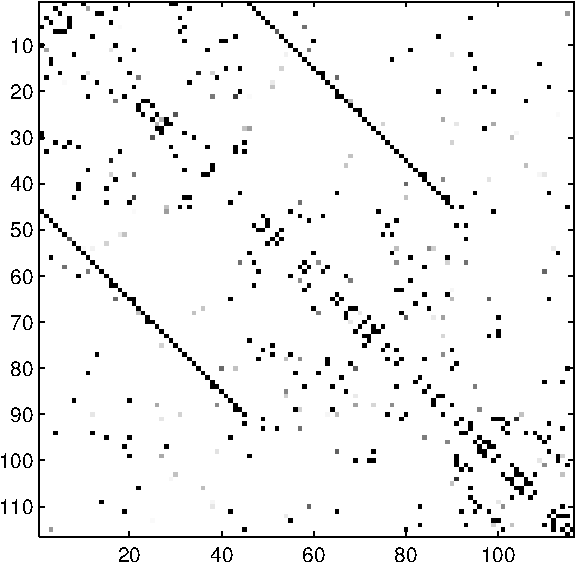
\includegraphics[height=0.28\textwidth]{images/new/struct_subj1-crop}
  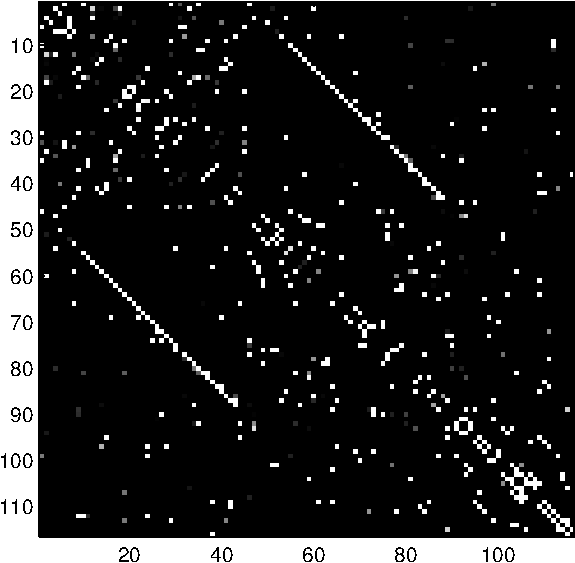
\includegraphics[height=0.28\textwidth]{images/new/struct_subj2-crop}
  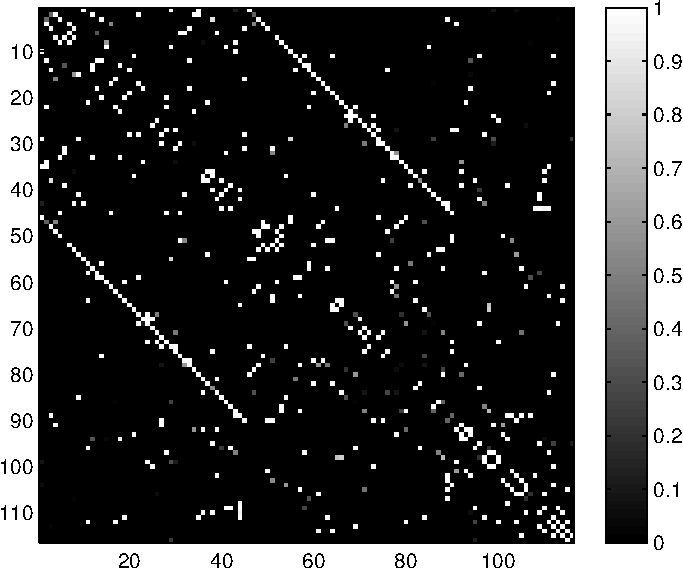
\includegraphics[height=0.28\textwidth]{images/new/struct_subj3_colorbar-crop} % one colorbar at the top right of the figure
  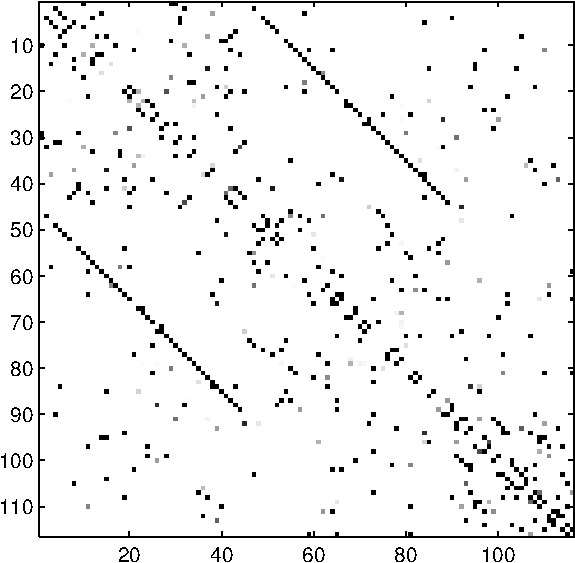
\includegraphics[height=0.28\textwidth]{images/new/struct_subj4-crop}
  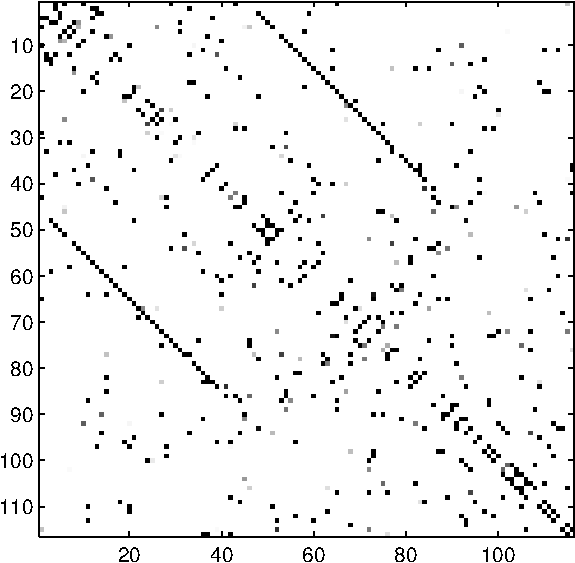
\includegraphics[height=0.28\textwidth]{images/new/struct_subj5-crop}
  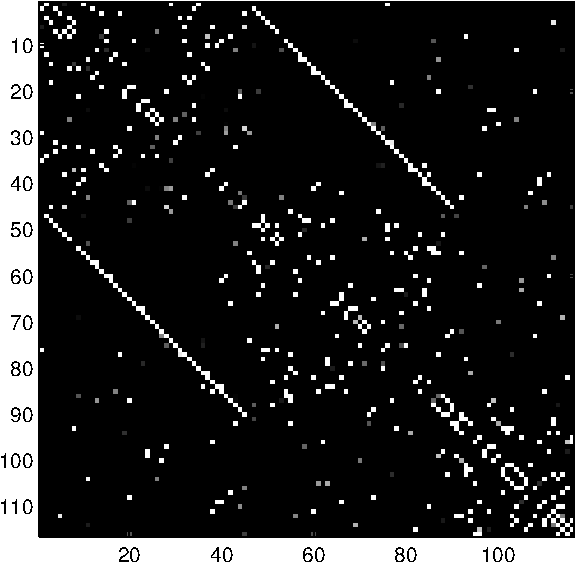
\includegraphics[height=0.28\textwidth]{images/new/struct_subj6-crop}
  \caption{The structure of all six subjects as found with the PC algorithm. The two diagonal lines represent connections between the two hemispheres.}
\label{fig:struct_subjects}
\end{figure}

\begin{figure}[h!]
  \centering
  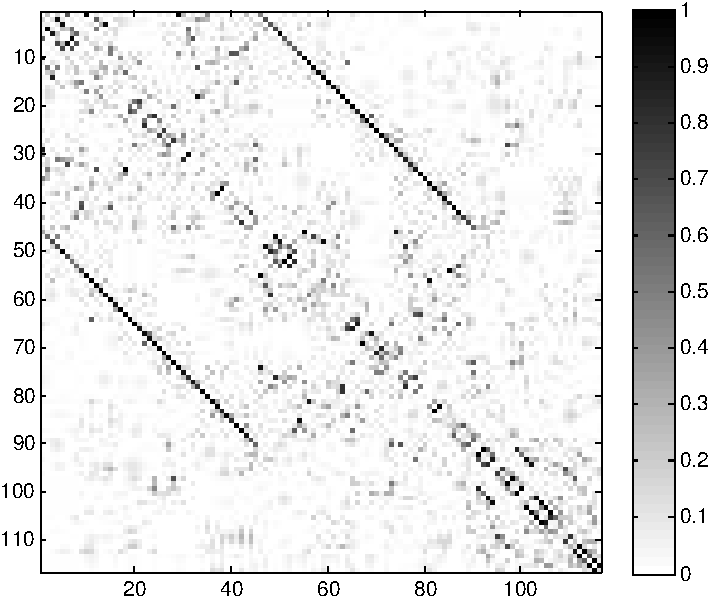
\includegraphics[width=0.49\textwidth]{images/struct_full}
  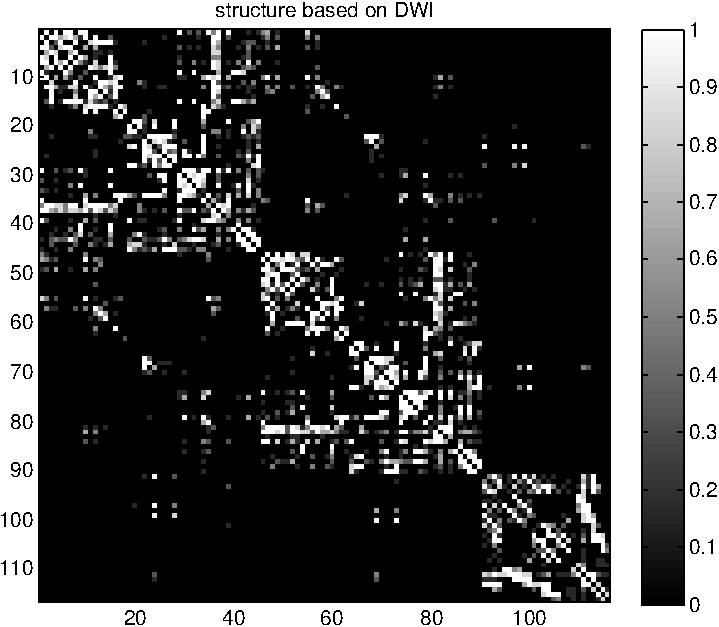
\includegraphics[width=0.49\textwidth]{images/structure_max}
  \caption{The avarage structure of all subjects. The structure on the left is found with the PC-algorithm, and the structure on the right is found with DWI-measurements by Hinne et al. The two diagonal lines represent connections between the two hemispheres.}
\label{fig:struct_avg}
\end{figure}

\subsection{Directed graphs}
This structural graph has been used as a basis for a directed graph, for both standard PC and EMS-PC.
As there were no notable differences between different subjects, only the average PDAG across all subjects is presented.
The results for standard PC and EMS-PC are shown in figure~\ref{fig:pdag_avg}.
Although many arrowheads are found with probabilities above 0.9 for both variants of the algorithm, the graph looks strongly symmetric.
In terms of causality, this means that many latent sources are still present and causal relations between the measured brain regions themselves are not clearly visible.

\begin{figure}[h!]
  \centering
  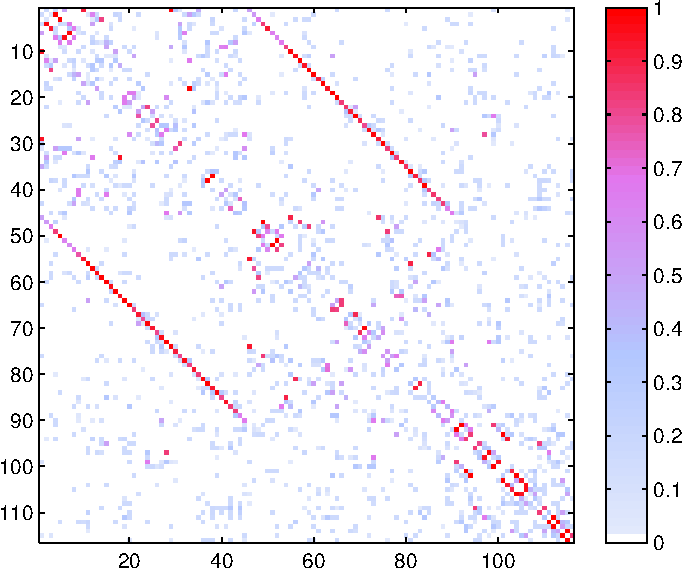
\includegraphics[width=0.49\textwidth]{images/new/PDAG_avg_mod-crop}
  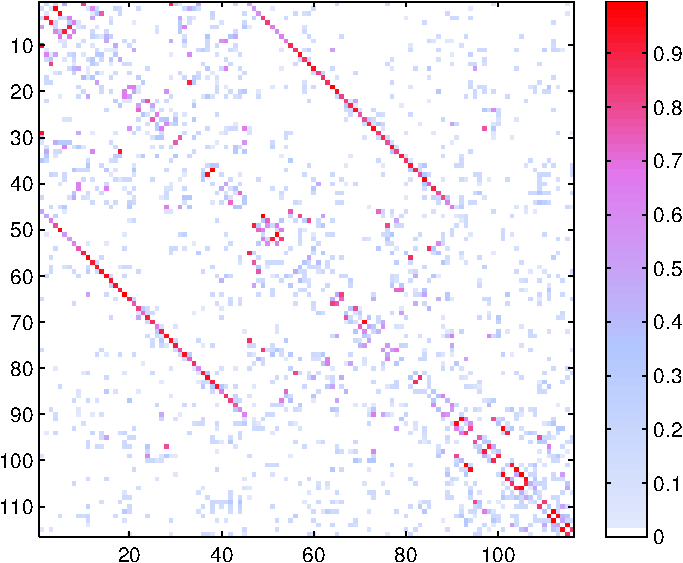
\includegraphics[width=0.49\textwidth]{images/new/PDAG_avg_expl-crop}
  \caption{The PDAG found standard PC at the left, and EMS-PC at the right. A high value denotes a high certainty of an arrowhead. The average of all six subjects is taken.}
  \label{fig:pdag_avg}
\end{figure}

Another representation of this data has been used to emphasise the asymmetric parts of the directed graphs.
To achieve this, the absolute difference between these matrices and their transpose has been calculated, lifting out those points for which there is an arrow in one direction, but not in the opposite direction.
These resulting antisymmetric matrices are presented per subject for EMS-PC in figure~\ref{fig:asym_subjects}. The average across all subjects for both variants of the PC algorithm are presented in figure~\ref{fig:asym_avg}.

\begin{figure}[h!]
  \centering
  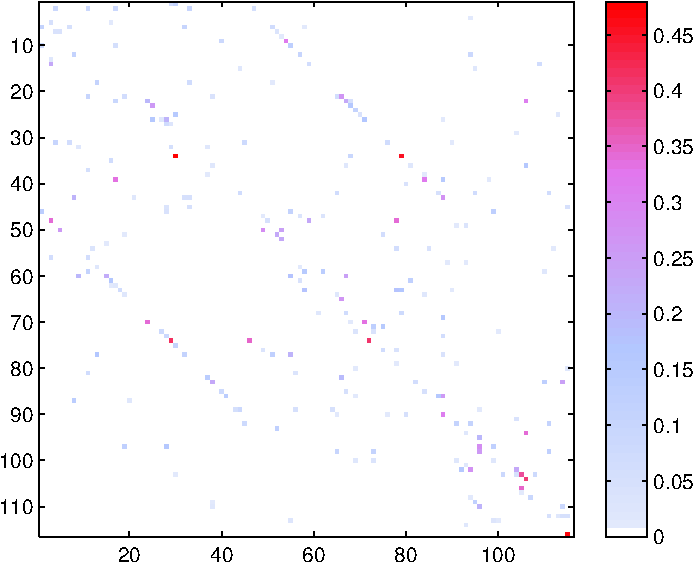
\includegraphics[height=0.25\textwidth]{images/new/assym_subj1_expl-crop}
  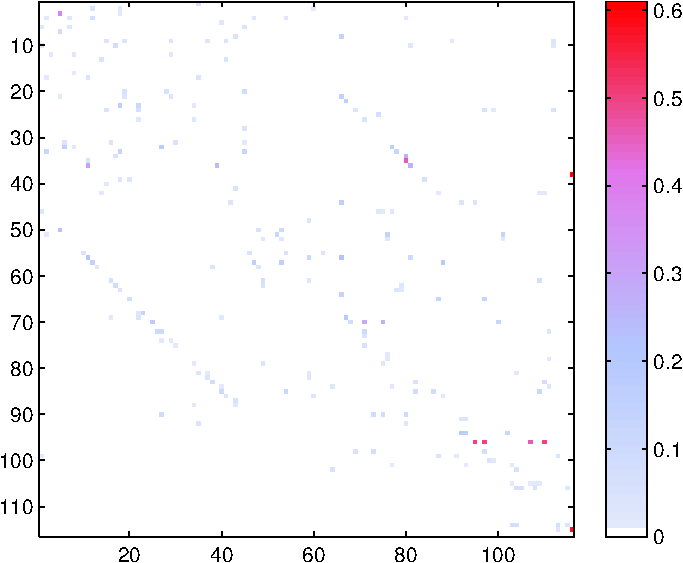
\includegraphics[height=0.25\textwidth]{images/new/assym_subj2_expl-crop}
  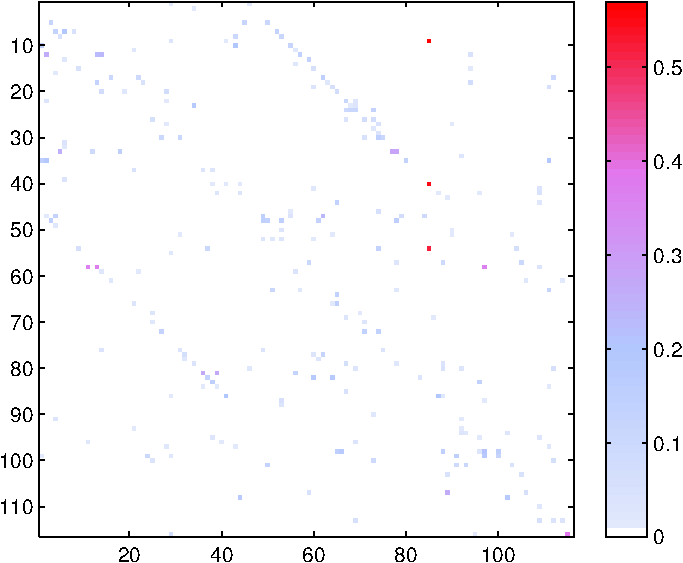
\includegraphics[height=0.25\textwidth]{images/new/assym_subj3_expl-crop}
  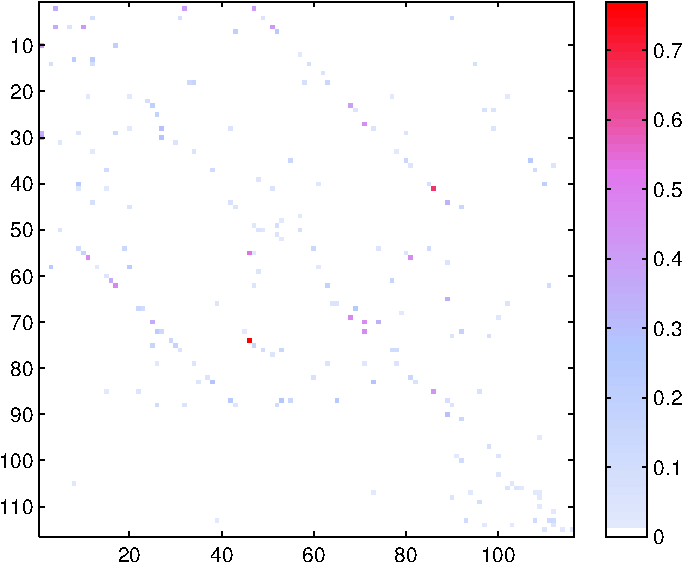
\includegraphics[height=0.25\textwidth]{images/new/assym_subj4_expl-crop}
  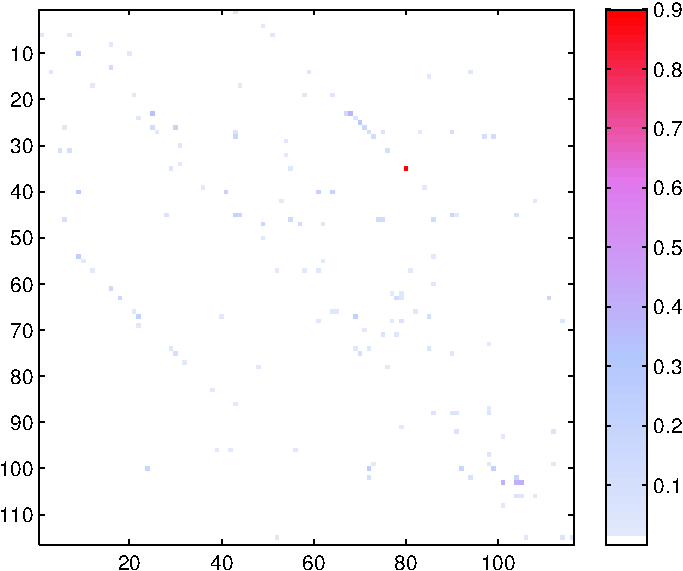
\includegraphics[height=0.25\textwidth]{images/new/assym_subj5_expl-crop}
  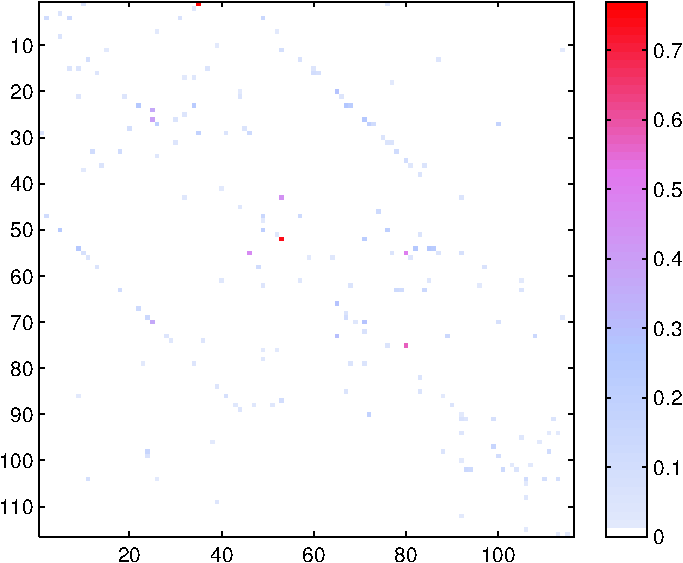
\includegraphics[height=0.25\textwidth]{images/new/assym_subj6_expl-crop}
  \caption{The assymetric parts of the PDAG found with EMS-PC for all six subjects, in which a high value denotes a high certainty of a one-directional arrow.}
\label{fig:asym_subjects}
\end{figure}

\begin{figure}[h!]
  \centering
  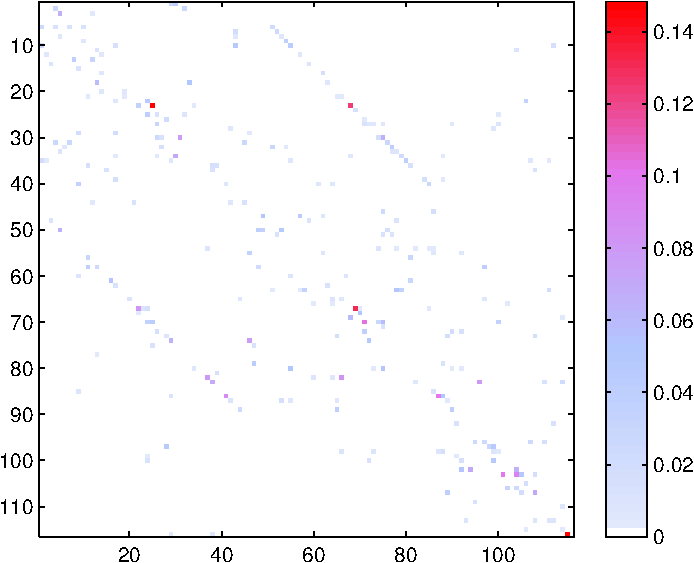
\includegraphics[width=0.49\textwidth]{images/new/assym_avg_mod-crop}
  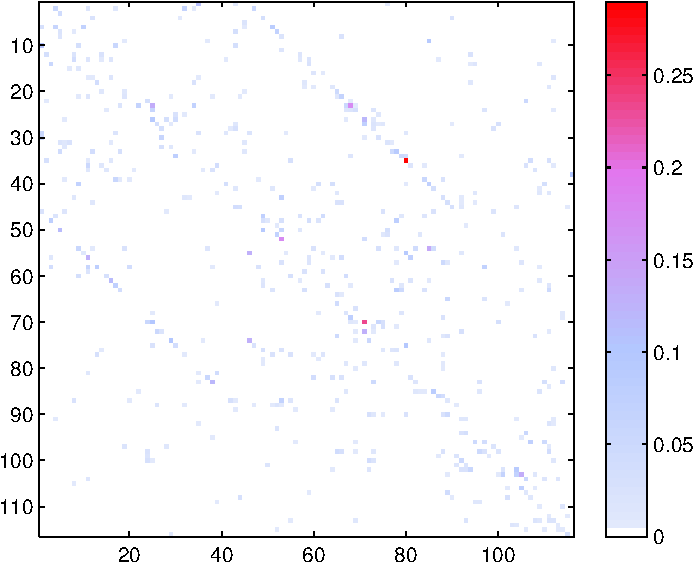
\includegraphics[width=0.49\textwidth]{images/new/assym_avg_expl-crop}
  \caption{The asymmetric parts of the PDAG found with standard PC on the left, and EMS-PC on the right. A high value denotes a high certainty of an one-directional arrow. The average of all six subjects is taken.}
  \label{fig:asym_avg}
\end{figure}

As can be seen in figures~\ref{fig:asym_subjects} and~\ref{fig:asym_avg}, the certainties of one-directional arrows are very low compared to the certainties of the bi-directional arrows. Also, the certainties of one-directional arrows are somewhat higher in EMS-PC than in standard PC.
For EMS-PC, the highest certainties found for one-directional edges per subject are in the range of 0.45 to 0.9, whereas the avarage across subjects has a maximum value of 0.3.
The few one-directional arrows found in idividual subjects therefore do not seem to be consistent across different subjects.

To illustrate the difference in certainties between bi-directional and one-directional edges, the distributions of these values are presented in figure~\ref{fig:distributions}.
\begin{figure}[h!]
  \centering
  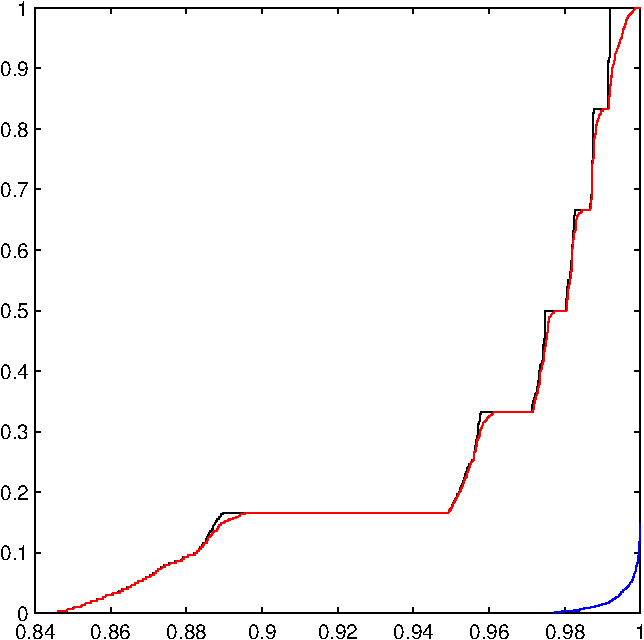
\includegraphics[width=0.49\textwidth]{images/new/dist_all_mod_blackstruct_reddir_blueantisym-crop}
  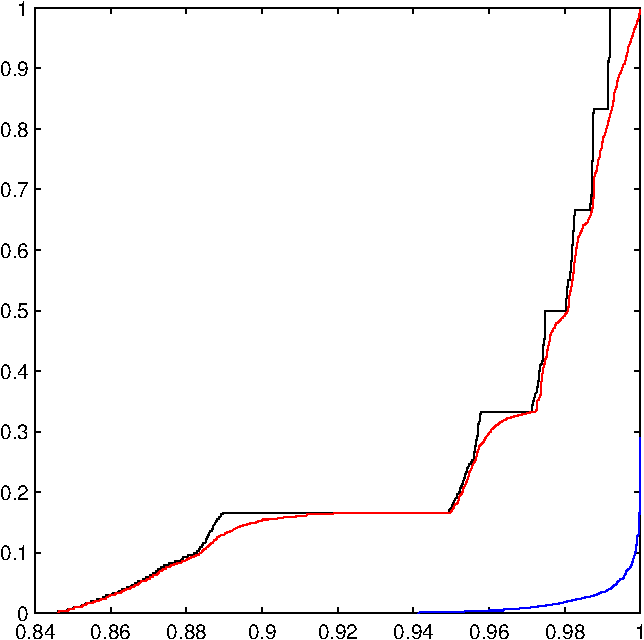
\includegraphics[width=0.49\textwidth]{images/new/dist_all_expl_blackstruct_reddir_blueantisym-crop}
  \caption{The distribution of values, for standard PC at the left, and EMS-PC at the right. The horizontal axis shows the relative number of occurences in the graph. Zero-values make up more than 84\% of the graph, these are not shown in this distribution. The black line represent the distribution of results of the structural part of PC, and is equal for both variants. The red and the blue line represent the distribution of values of arrowheads and one-directional arrows, respectively.}
  \label{fig:distributions}
\end{figure}
 
\subsection{Execution time of the algorithm}
To apply the algorithms on our data, we have used a Xeon E5-2670, running on 2,6GHz.
To run one iteration of the PC algorithm for one subject, modified PC needed approximately one minute and EMS-PC needed approximately two minutes to find both structure and direction.
Although PC is not designed to be multithreaded, running multiple iterations lends itself for using multiple threads, as the iterations are fully independent, and only need to be averaged out afterwards.

\section{Discussion}
%Good consistency of structure within and between subjects
Many structural connections found by the PC algorithm are found consistently, both within one subject and also across multiple subjects.
The connections between the two hemispheres can clearly be seen in all subjects, as well as many connections in the corpus callosum.
The consistency can also be seen in the distribution of values in figure~\ref{fig:distributions}.
Non-zero values make up approximately 16 percentage points of the graph, of which 3 percentage points show a certainty larger than 0.5.
Approximately 1 percentage point even shows a certainty of 1.

% TODO: Maak duidelijk welke aannames gedaan worden in welke PC variant en welke aannames verzwakt zouden kunnen worden.

% Quick run-time
For PC as well as standard PC we were able to run hundreds of iterations on 116 variables in a matter of hours per subject.
Iterations can also be run in parallel.
Further speed increments can be achieved by coding the algorithm in a low overhead language.

%Comparison with DWI inter-hemisphere connection
Standard PC and particularly the first, structural part, definitely has similarity with respect to existing methods based on DWI.
This is not completely surprising as standard PC yields a functional network and DWI based methods yield anatomical structural networks, two network types which are tightly related.
A less apparent observation is the clear presence of correlation between homologous area's in the functional network, which lacks in the structural network as found with DWI.
An explanation to this difference might be that these correlations respond to the long white-matter tracts connecting the two hemispheres through the corpus-callosum.
It is known that DWI has difficulty in measuring such long tracts, while the presence of correlation between two connected ends cannot be argued against.
As such, statistical baed causal discovery methods contribute additional information to finding structural connectivity.

% Comparison Markov class standard PC and EMS-PC
Both standard PC and EMS-PC find many bi-directional arrows, with some one-directional arrows.
As can be seen in the distribution of values in figure~\ref{fig:distributions}, nearly all found edges are oriented as bi-directional arrows.
For EMS-PC, this number is somewhat lower but there are still few one-directional arrows, and they do not have certainties higher than 0.15.
These certainties are not high enough to conclude any causal relations.

%Poor consistency of directionality between subjects
There is some significant and consistent directionality within each of the subjects.
However the variance of this directionality between subjects is so high, there is no significant consistent one-directionality between them.
We were unable to find existing literature on connectivity methods regarding significant intra-subject one-directionality.
%Lack of symmetry
There is also little to none symmetry in directionality between the two hemispheres within and across subjects.
One would at least expect some symmetry to be found.
This demonstrates that the gap between analytical methods for effective connectivity and anatomical correctness is still too wide.

% Further research
Further research may be done to investigating whether any of these arrows have a physiological meaning.
This can be done by repeating these experiment with more subjects to get a better view on the significance of the directional edges.

%HRF
One main strength of a general causal discovery method is that fluctuations in haemodynamic respons do not pose a problem.
To continue this type of research, other causal discovery methods might be also be applied, and attempts can be made to negate the disadvantages of the PC algorithm.

A causal network or Bayesian network cannot contain cycles by definition.
However, exclusion of cycles in brain networks has not been proven and also seems unlikely.
We believe an interesting direction of further research would be to apply cyclical causal methods, such as the method proposed by Mooij and Heskes\cite{Mooij20013}.

We believe application of a Bayesian approach will provide a better insight.
Standard PC and EMS-PC lack a robust measure of uncertainty.
There is no baseline or correctness measure to compare results or data with
A Bayesian approach such as proposed by Claassen and Heskes will provide more slack and insight in results \cite{claassen2012}.
This in turn will leverage development of better and faster data driven methods.


% TODO: Suggereren task based analysis ipv resting state voor beter causaal beeld. 

%cause of poor consistency: inherent to our method or viable for further research?

% \section{Conclusion}
%repeat everything in 1 paragraph, or leave away, whatever seems most fitting in the end. HRF makes us awesome


\bibliography{references}{}
\addcontentsline{toc}{section}{References}
\bibliographystyle{plain}


\end{document}